\startchapter{Methodology and Constructs}
Before we dive into our actual studies of the effect of socio-technical congruence and its use to form recommendations, we will go through some common definitions (Section~\ref{}) and constructs (Section~\ref{}) that are necessary to clarify for the remainder of the thesis.
Furthermore, we also will discuss the general approach to the data collection methods employed (Section~\ref{}) as well as our analysis methods used (Section~\ref{}).

\section{Definitions}
We sill start with defining three constructs that we are heavily relying upon: (1) Work Item's being a complete unit of work, (2) Change-set being the technical work submitted by a developer, and (3) builds referring to a testable product.

\subsection{Work Item}
A \emph{Work Item} is a unit of work that can be assigned to a single developer.
These units of work can span anything from single bug-reports, reported by either the end user or by a developer, to feature implementations.
These \emph{Work Item}s can be hierarchically organized in order to broken down into more manageable pieces.
Still one developer or better one project team member is responsible for a work item to be completed, the sub work items that break it down do not necessarily be assigned to the owner of the parent work item.

For instance, in the case of the IBM Rational Team Concert development team creates story items to describe larger functionality from the user point of view and assigns depending on the complexity and implication of the story to a component or team lead, or a developer.
The owner of the story then either breaks down the story into multiple stories or tasks which are again assigned to team members according to their complexity and implications.
Once the work item level is sufficiently low the developer assigned to it can make the necessary modification to the project to close the work item.

\begin{note}
\begin{mydef}
A \emph{Work Item} is a defined and assignable unit of work.
\end{mydef}
\end{note} 

\subsection{Change-Set}
A \emph{Change-Set} is a set of source code changes applied to a number of source code entities, with an entity being the artifact that a developer would change to add to, modify, or delete from the current product. that are by the developer bundles into one set.
For example, in the Eclipse project\footnote{www.eclipse.org} the developer use CVS\footnote{} as their version control system to manage changes to the Eclipse IDE.
A developer will check out her current version of the repository and started editing, creating and deleting files in order to fulfill a work item she is currently working on.
Once the developer decides that she accomplished the work to finish her current work item, she commits her changes.
Those changes that consists of file creations, deletions and modifications taken together are referred to as a \emph{Change-Set}. 

\begin{note}
\begin{mydef}
A \emph{Change-Set} is a set of modifications, additions and deletions of software artifacts such as source code files, classes or methods.
\end{mydef}
\end{note}

\subsection{Build}
The goal of each software development team is to deliver a finished or improved product at some point in time.
This finished product is often referred to as the final \emph{Build}.
A \emph{Build} can generally be referred to as any instance of the product that can be run to some extend.
To create a build a team gathers all the changes to work items describing changes that are required for the new build and compiles and packages the product.
The amount of work items and their respective changes included in a build will gradually increase over time because more work will be finished as the project progresses.

In the case of the IBM Rational Team Concert development team, they create builds on a frequent basis to test the product as a whole to look for integration issues. 
The team also subscribes to the philosophy to use their own products as intensely as possible themselves and thus try to bring each build to a level that it can be used continuously for development.
This intense use enable the team to spot issues that are still within the product and better asses the severity of those found issues.

\begin{note}
\begin{mydef}
A \emph{Build} is a to some extend executable version of the product that includes a number of changes implementing work items.
\end{mydef}
\end{note}

\section{Constructs}
From the definitions we are working with we can derive the three central constructs we work with in this thesis: (1) the social network connecting communicating and coordinating developers, (2) the technical network connecting developer that are dependent through code artifacts, and (3) the socio-technical network that combines the social and technical network in a meaningful way.
This sections draws heavily from our work done in collaboration with Timo Wolf, Daniela Damian, Lucas Panjer, and Thanh Nguyen~\cite{wolf:ieee:2009}.

\subsection{Social Network}
\begin{figure}[t!]
\begin{center}
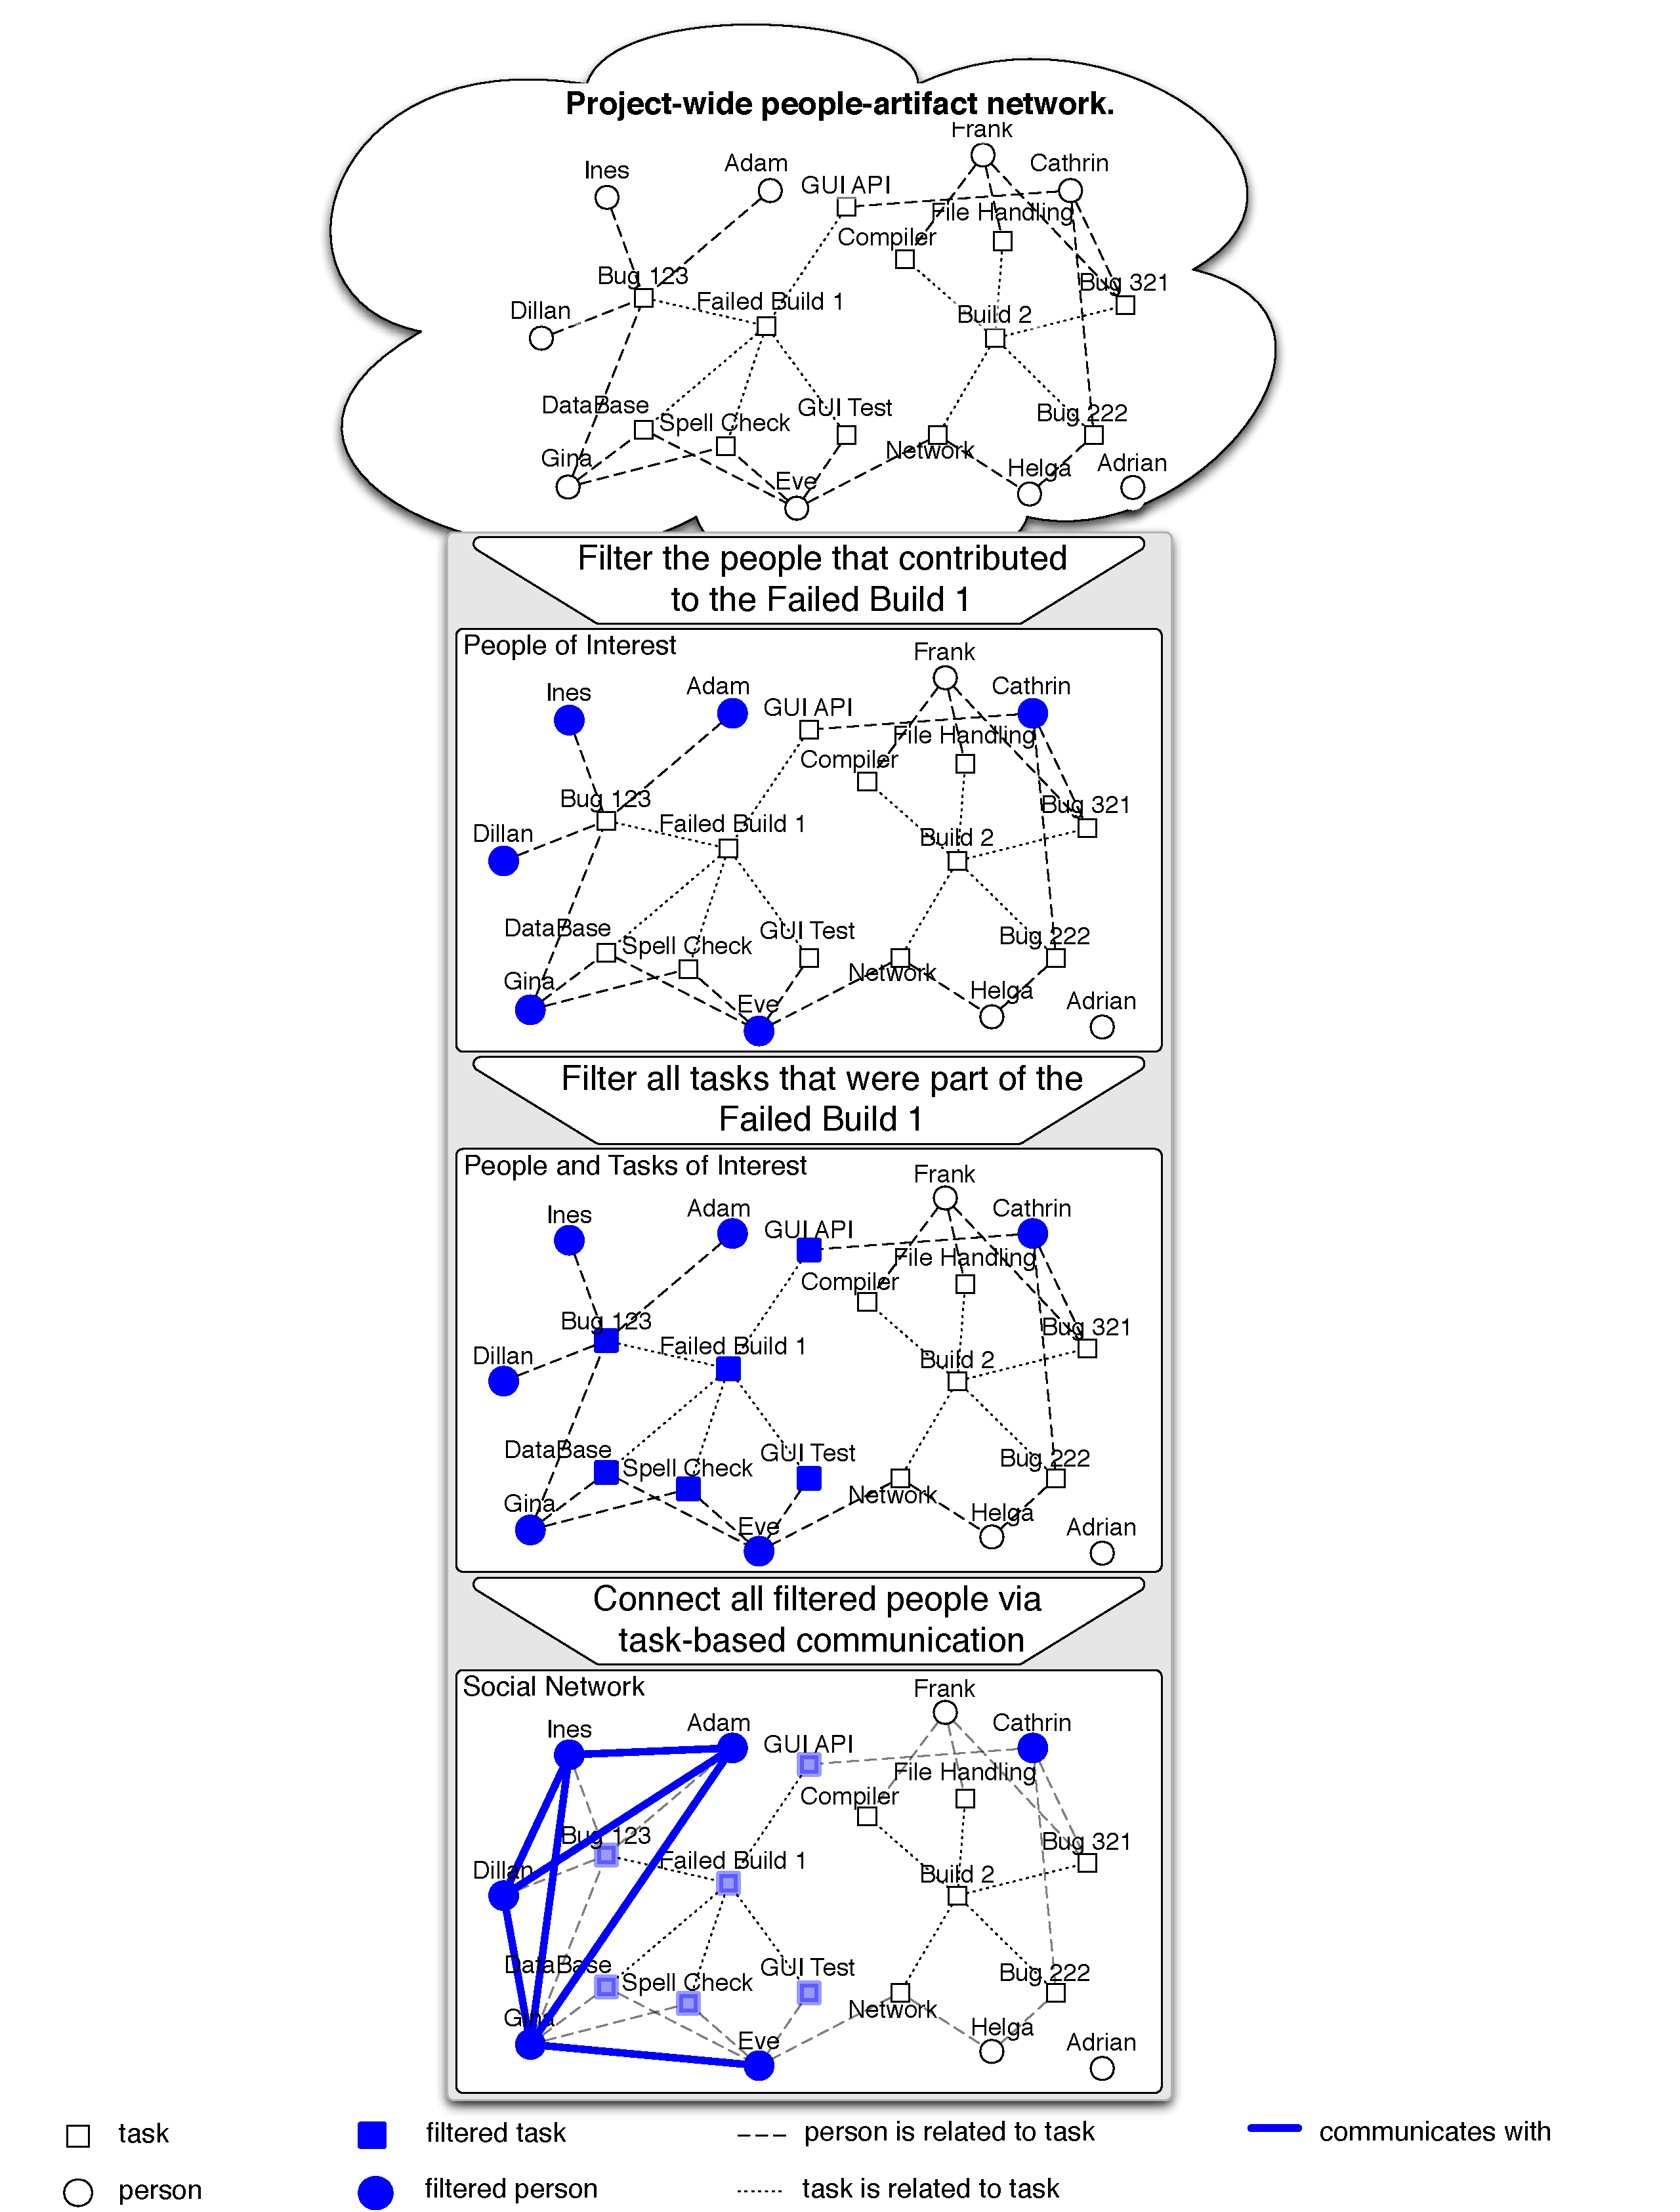
\includegraphics[height=1\textwidth]{./figures/grand_figure}
\caption{Social network construction examples in our approach}
\label{fig:network}
\end{center}
\end{figure}
To illustrate our approach to construct social networks we go through the example to help solve team collaboration problems, by following the example of a failed build (left side of Figure~\ref{}). 
A social network is represented as a graph that consist of nodes connected by edges. 
In our approach, the nodes represent people and edges represent task-related communication between these people.

Let us start with a high level description of how we conceptualize and construct social networks for software teams. 
The approach is repository and tool independent and can be applied to any repositories that provide information about people, tasks, technical artifacts, and communication. 
This include work, issue, or change management repositories, such as Bugzilla or IBM Rational Team Concert; or source code management systems, such as CVS or IBM Rational Team Concert; or even communication repositories such as email archives.

We construct and analyze social networks within a \emph{collaboration scope} of interest.
With a collaboration scope defining the people and interactions of interest.
In this example, around Failed Build 1, the collaboration scope is the communication of the contributors to the failed build. 
Other examples include the collaboration of people working on a critical task, in a particular geographical location, or in a functional team such as testing.

There are three critical elements that are necessary to construct task-based social networks for a collaboration scope and that need to be mined from software development repositories:

\begin{description}
\item[Project Members] are people who work on the software project. 
These \people s can be developers, testers, project managers, requirements analysts,
or clients. 
Project members, such as Cathrin and Eve, become nodes in the social network.

\item[Work Items] are units of work (as defined earlier) within the project that may create a need to collaborate and communicate about. 
Examples for a work item include resolving Bug  123 or implementing the GUI API. 
More generally, implementing feature requests and requirements can also be considered collaborative tasks.

\item[Work Item Communication] is the information exchanged while completing a work item and is the unique information that allows us to build task-based social networks. 
In our example, dashed black lines represent task-related communication such as a comment on Bug 123, or an email or chat message about GUI API.
Task-related communication is used to create the edges between developers in the social networks.
\end{description}

The data underlying the social network constructed used throughout this thesis are based on work items and their associated discussions.
In IBM Rational Team Concert each work item has an attached discussion threat were developer can discuss the work item or simply note down their thoughts while working on the work item.
This means, we would create a link between two developer if they comment together on the same work item to indicate that they are part of the same discussion.

\subsection{Technical Network}
\begin{figure*}[t!]
\centering
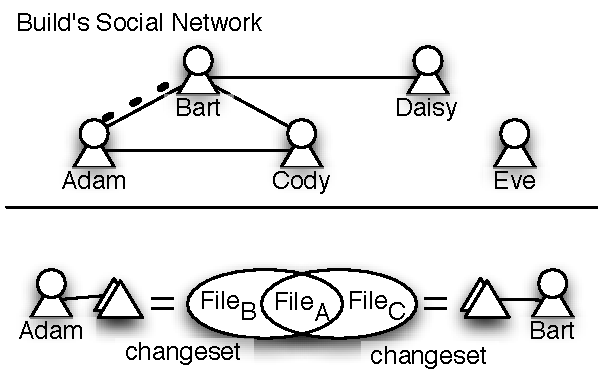
\includegraphics[width=.7\textwidth]{figures/addedge}
\caption{Creating a technical network by connecting two developer that changed the same file.}
\label{fig:addtechnicaledge}
\end{figure*}

% some preamble as in the previous subsection
Building technical networks follows a very similar approach we described for building social networks.
In fact the technical network is a social network whose only main distinction from the social network described earlier lies in the way edges between nodes are based on.
We derive the name of technical network from the way we link developer with each other, namely if they are modifying related source code artifacts.
As in the previous network construction, the construction of the technical network is based on three components:

\begin{description}
\item[Project Members] are people who work on the software project. 
These \people s can be developers, testers, project managers, requirements analysts,
or clients or in general anyone that modifies software artifacts through change-sets. 
In Figure~\ref{} project members, such as Adam and Bart, become nodes in the technical network because they modified the same file.

\item[Change-Sets] are changes made to software artifacts by individual users. 
A set consists of a number of artifacts that have been modified as well as the modifications themselves.
For example Adam as shown in Figure~\ref{} modified File$_{\text{A}}$ and File$_{\text{B}}$.

\item[Software Artifact Relation] describe the relation between developer in the technical networks.
These relationship can be defined in several different ways.
For example, in Figure~\ref{} Adam and Bart are related through a technical relationship because they modified the same file.
Note, that we are mostly interested in relationship between artifacts that are effected by changes.
\end{description}

% Example as shown in the picture
Constructing social networks therefor follow three steps: (1) we gather all the change-sets of interest, (2) identify the relations between artifacts, (3) infer from the change-sets and the relations between the source code artifacts the relation between the artifact owners.
For example, after we selected the set of change-sets of interest we define the change-sets themselves as the source code artifact and identify the owners of those artifacts.
Then we infer the relationship between those source code artifacts by relating all change-sets that changes the same source code file.
And as Figure~\ref{} shows this means in the case for Adam and Bert that they are connected because both own a change-set each that modifies a common file.

\subsection{Socio-Technical Network}
\begin{figure}[t!]
%	
  \centering
  \subfloat[Inferring to the build focus relevant change-sets and work items.]{
    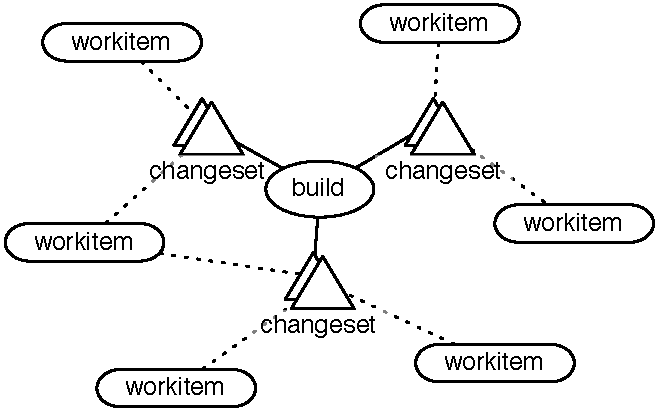
\includegraphics[width=.46\textwidth]{figures/buildworkitem}
    \label{fig:construct-focus}
  }
 % 
  \hspace{8pt}
  \subfloat[Constructing an social networks from work item communication.]{
	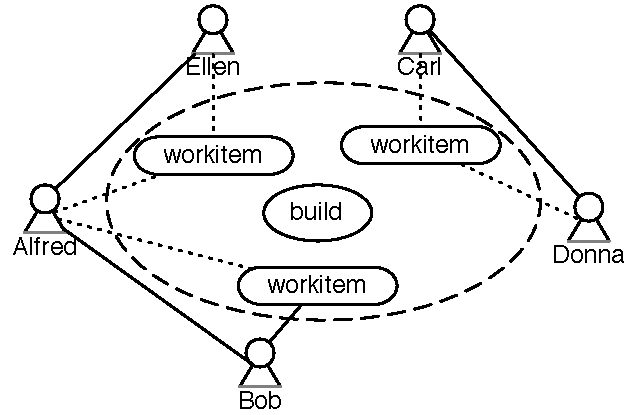
\includegraphics[width=.46\textwidth]{figures/buildsn}
     \label{fig:construct-sn}
  }
  
    \subfloat[Linking developers in a technical networks via change-set overlaps.]{
  	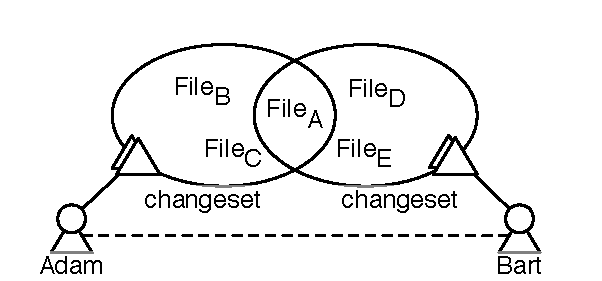
\includegraphics[width=.46\textwidth]{figures/cochangedfiles}
    \label{fig:construct-tn}
  }
  %
    \hspace{8pt}
  \subfloat[Combine social and technical networks into a socio-technical network.]{
  	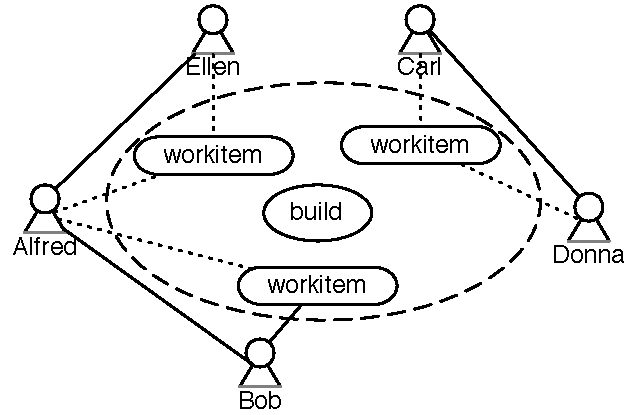
\includegraphics[width=.46\textwidth]{figures/buildsn}
	\label{fig:construct-combine}
  }
  \caption{Constructing socio-technical networks from IBM Rational Team Concert data.}
  \label{fig:construct-stc}
\end{figure}

Socio-Technical networks are a meaningful combination of both social and technical networks.
Selecting this meaningful combination reflects itself in the selection of the work-items in the case of building the social network and selecting the change-sets and their relations in the case of the technical network.
Hence constructing a socio-technical network requires the following four steps:

\begin{enumerate}
\item\textbf{Selecting the Focus} used for the socio-technical network represents the glue that binds the social and technical network into a socio-techncial network. 
This focus also referred to as filter in our earlier publication~\cite{}, determines the content of the networks.
One example we will use in this thesis for the focus of such networks are software builds to construct networks that are describing the coordination among developer for a given software build.
\item\textbf{Constructing the Social Network} follows the description above with the focus determining the work items that are selected to generate the nodes from the work item participants and the edges from the communication among the participants through a work item.
\item\textbf{Constructing the Technical Network} follows the description of constructing technical networks above with the focus determining the change-sets being used to determine and connect developers in the network.
\item\textbf{Combining Networks} is the final step that overlays the networks by unifying the set of developers in both networks.
Thus a pair of developers can be directly connected with each other through two edges, one representing the edge from the technical network and the other the edge from the social network.
\end{enumerate}

% describe the example in the figure
Figure~\ref{fig:construct-stc} shows an example on how we in our studies of the IBM Rational Team Concert development team used to create socio-technical networks.
In the first step (Figure~\ref{fig:construct-focus}) we set the focus to be a software build which allows us via the change-sets that made it into the build to infer what work items are also represented in said build, by following the link between a change-set and a work item.
Given the focus, constructing the social network can be constructed using the work items that can be linked to the software build (Figure~\ref{fig:construct-sn}).
Similarly the construction of the technical network relies on the change-sets that went into a build. 
To actually infer edges between developer, we relying on co-changed files within a build as an indicator of work dependency (Figure~\ref{fig:construct-tn}).
Finally, the two networks are combined and yield the socio-technical network shown in Figure~\ref{fig:construct-combine}.

\section{Data Collection Methods}
To conduct the research for this thesis we drew upon multiple data sources.
In order to get a picture across the whole development history of the IBM Rational Team Concert development team and other projects we studied we employ repository mining techniques to identify larger trends in measurable activities.
In oder to gain a more in-depth understanding on how developers actually work and deal with interdependencies especially how they would react to certain recommendations and whether they are can be made useful we employ qualitative methods.

\subsection{Repository Mining}
Software development usually employs several software repositories.
Those repositories can be the version control archives tracking changes made to the software system, they also can be issue or task management software to keep track of issues that need to be resolved and features that need to be implemented.
Additionally, those software repositories can also contain digital communication such as forum and email discussions or log of IRC\footnote or instant messenger chats.

Those repositories can grow to considerable sizes depending on the projects live span and intensity. 
Therefore, it is often infeasible for an individually to review the history for a whole project and it is necessary to employ data-mining techniques to be able to analyze trends within those repositories.
Although this approach is limited in helping to gain a deep understanding of the intricacies of a development project it nevertheless is invaluable to place in-depth results in the bigger picture of the project.
Furthermore, data mining approaches are one way to easily feedback value to the development team without burdening any individual developer with diverting time to other non automatic data collecting instruments.
This is an important point as one goal of this thesis is to explore the ability of the concept of socio-technical congruence to generate actionable recommendations.
In case a developer needs to personally provide a large amount of information manually the overhead generated by a system might outweigh the benefit of recommendations and therefore make them useless.

We therefore extract information from three different types of repositories: (1) version control, (2) task management, and (3) build engine.
The version control supplies us with the knowledge on how developers are connected through their technical work.
The task management supplies us with the information on who communicated with whom with respect to a work item.
And lastly the build engine supplies us with the focus to construct socio-technical networks.

In order to derive socio-technical network we will need to link the different artifact types.
Within IBM Rational Team Concert as illustrated in Figure~\ref{fig:construct-focus} work items are linked to change-sets and change-sets are linked to builds, therefore, establishing the connections needed to construct socio-technical networks with a build as focus.
Similarly these links can be inferred as proposed by Cubranic et al~\cite{cubranic:tse:2005} from repositories that are missing the capabilities of creating formalized links.

Note, we will provide more detailed in the respective studies on how we employed repository mining techniques.

\subsection{Surveys}
To complement the insights we obtained from the repository mining we first opt to deployed surveys with the entire RTC team at the end of our observation period. 
Surveys are designed iteratively and piloted before deployment, and intended to collect input to enrich and clarify information obtained from the software repositories. 
With each survey we try to minimize the time each developer needs to spend completing them, which usually limits ourselves to focus on closed questions offering prepared answers.
We constrain ourselves in this way to minimize the distraction to each individual developer in order to increase the response rate.

Our surveys are deployed through web services to make the collections more convenient to each developer as they are spending most of their times working at a computer enabling them to fill in the survey at their earliest convenience instead of keeping track of a paper version that might not easily be returned, especially considering that the development teams we are collaborating with are distributed across different continents.

Note, we will discuss the actual surveys we employed during our studies in the respective chapters as well as the target population, the population size, and the response rate.


\subsection{Observations}
The next richer and also to the developer more distracting method of data gathering are observations.
Although not necessarily actively interrupting and distracting developer, the act of observing can distract developers and also change their behaviour.
In order to minimize this type of distraction and the mitigate the observer bias, we employed a special form of observation study.
In short we became both an observer and a participant.
%
Being a participant has a multitude of advantages:

\begin{itemize}
\item\textbf{Reciprocity.} By participating in the actual development we can actually provide value to the development team from the very beginning.
This, in turn, motivates the developers to give us the time we need to conduct other parts if the study, like surveys and interviews, because they know that we already gave them something in return independent of the findings of our study.
\item\textbf{Learning the Vocabulary.} Each development project has its own project vocabulary~\cite{} in order to efficeively and cleary communicate. 
Understanding this vocabulary as an outside is not necessarily easy but very important to make sense of comments and answers supplied in interview and survey and of course to better interpret observations made such as of discussions among developers.
\item\textbf{Understanding the Context.} For example in one study our observation period coincided with the months prior to a major release and during which the team focused on extensive testing rather than new feature development. 
% something about the context helping
Because of this closeness of our observation period to a major release we observed mainly activities around integration testing with little coding activity aside from fixing major bugs.

Although it is easy to ascertain when the next major release of the product is, the effect this has on the developer besides a change in the process is harder to gauge.
Being part of the development effort hows more clearly how developer react to the change in process and better understand their struggles.

\item\textbf{Asking more Meaningful Questions.} Having better understanding of the project and how it affects the individual developer as well as understand the vocabulary they use helps with phrasing better questions.
Better in the sense of both more meaningful to the developer and in the sense of understandability because they can be phrased using the project vocabulary.
\end{itemize}

Besides of gaining a better understanding of some easily missed or miss-understood intricacies, working together with the developer establishes a trust relationship~\cite{}.
This trust helps to mitigate observation biases that are introduced by simply observing as well as makes developers more forthcoming during interviews and surveys~\cite{}.
As you notices it is hard to separate the different data collection methods that involve human interaction, therefore we think combining these data collection methods in the right order can greatly enhance the data collected.


\subsection{Interviews}
We conducted interviews with ten developers of the RTC team to inform our observational findings. The setting for the interviews was slightly unusual, and beneficial from a research perspective, since the first author's participant-observation allowed him to develop working relationships during his stay at the team, and to delve into a discussion of complex communication issues without needing to spend time understanding the basic context of the team.

In the interviews, we requested developers to provide details into their communication dynamics through a narration of ``war stories'' that directly related to communication among developers. ``\emph{War stories}'' are events that left an impression on the respondent. War stories emphasize specific events that they witnessed or took part in~\cite{lutters:ist:2007}; their narrative is particularly powerful at uncovering the elements of the stories that are relevant to the respondents. The interviews lasted between thirty minutes and one hour, and they were conducted at the end of the observation period. 


\section{Analysis Methods}
\subsection{Statistical Analysis}
\subsection{Grounded Theory}













